\documentclass{standalone}
\usepackage{pgfplots}
\pgfplotsset{compat=1.16}
\begin{document}

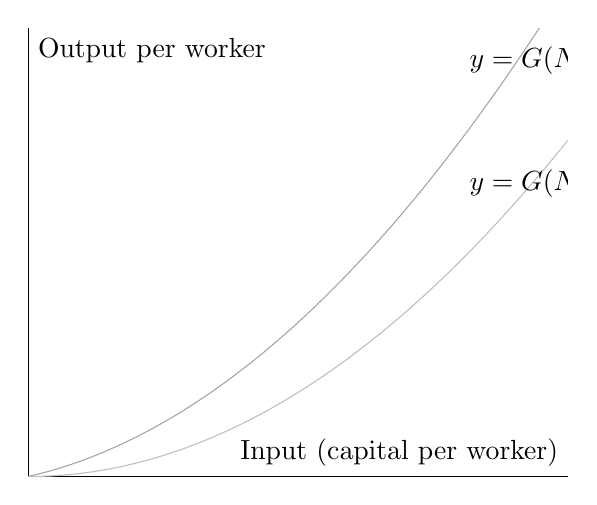
\begin{tikzpicture}
    \begin{axis}[
        axis lines=center,
        xlabel={Input (capital per worker)},
        ylabel={Output per worker},
        xmin=0, xmax=10,
        ymin=0, ymax=4,
        xtick=\empty,
        ytick=\empty,
        enlargelimits=false,
        axis line style={-},
        tick style={black}
    ]
        % Plot for G(N)
        \addplot [
            domain=0:10, 
            samples=50,
            color=gray!50
        ] {(x/10)*(3*x/10)};
        \node at (8, 2.4) [above right] {$y = G(N)f(k)$};

        % Plot for G(N')
        \addplot [
            domain=0:10, 
            samples=50,
            color=gray!70
        ] {((1.1*x)/10)*((3*x/10)+1)};
        \node at (8, 3.5) [above right] {$y = G(N')f(k)$};
    \end{axis}
\end{tikzpicture}

\end{document}